\documentclass[a4paper,11pt]{report}
\usepackage{fullpage}
%\usepackage{cite}
\usepackage{lmodern}
\usepackage[T1]{fontenc}
\usepackage{textcomp}
\usepackage{xcolor,graphicx} % Future use
\usepackage{caption}
\usepackage{hyperref}
\usepackage[all]{hypcap}
\hypersetup{colorlinks=false, pdfborder={0 0 0}}
\usepackage{multirow}
\usepackage{amsmath}
\usepackage{tikz}
\usetikzlibrary{calc,backgrounds,positioning}
\usepackage[numbers]{natbib}
\usepackage{amsfonts}
\newcommand{\tickYes}{\checkmark}
\usepackage{pifont}
\newcommand{\tickNo}{\hspace{1pt}\ding{55}}
\usepackage{listings}
%\usepackage{algorithmic}

\begin{document}

\pagestyle{plain} % just page numbers at the bottom
\title{Pointcloud Cleaning}
\author{Rickert Mulder}
\maketitle

\begin{abstract}
Your abstract goes here, your abstract goes here, your abstract goes here, your abstract goes here, your abstract goes here, your abstract goes here, your abstract goes here, your abstract goes here, your abstract goes here. \cite{Bartels2001}
\end{abstract}

\tableofcontents
\newpage

\chapter{Introduction}

\section{Research question}


\section{System overview}


\section{Outline}
Explain what is discussed in the following chapters


% Motivation & research question
% Ethics
%!TEX root = thesis.tex
\chapter{Background} \label{ch:background}

% \todo[inline]{Lots more citations, preferably state that it's someone else's work, cite and then write about it.}

In this chapter, laser scanning and the 3D-reconstruction pipeline are introduced. In section~\ref{sec:heritage} the heritage preservation context for this work is laid out. In section~\ref{sec:scanners}, 3d scanning is introduced and is followed by a description of the process by which raw scanner data transformed into a model in section~\ref{sec:pipeline}. The chapter is concluded with a discussion of point cloud the cleaning process in section~\ref{sec:cleaning}.


\section{Digital heritage preservation} \label{sec:heritage}

Architectural heritage sites in many parts of the world are deteriorating or are under threat of destruction. The demolition of the Buddhas of Bamiyan by the Taliban in 2001 \cite{Toubekis2009} is a recent example of such an event. Such threats highlight the need to digitally preserve heritage sites in order to keep a historical record after sites are gone or weathered. Preservation efforts have utilised many techniques to record buildings and ruins. Early efforts made use of tape measures and theodolites to produce simple ground plans. More recently, photogrammetry lets geomaticians produce 3D models \cite{Heritage}. Laser range scanning is the latest technique that allows archivists to create extremely high resolution 3D models.

 % \todo{Patrick: need more general background: projects? other todr? photo/text archiver? say why they are no longer used}

% \subsection{Laser scanners}

% \todo{expand, say more, justify focus on laser scanning}
% \todo[inline]{What is a range scanner, what is a point cloud, what is a range scan?}

\section{3D scanning} \label{sec:scanners}

3D scanners are optical devices that capture the shape, position and appearance of real world objects. At the very least a 3D scanner will record coordinates of points on scanned surfaces. Gray scale or colour information may also be included. There are many types of 3D scanners on the market today. Each scanner has properties that make it more of less suitable for various scanning tasks. Generally, the size of the object and the level of detail one wishes to capture will determine ones choice of technology. Secondary factors such imaging speed, portability and cost of a scanner may also be important.

3D scanning technologies can generally be classified into two categories, namely triangulation and time of flight scanners.

\subsection{Triangulation scanners}

Triangulation scanners, as the name suggests, uses trigonometric triangulation \cite{Frohlich2004} to locate surface points in a scene. Triangulation scanners are primarily available in two flavours, those that use laser light and those that use white light \cite{Brown2012}. Laser triangulation scanners emit pulses that are reflected by an object and recorded by a sensor at a known position relative to the pulse origin. The sensor directly measures the angle of the returned beam that can then be used to compute the position of a point on an object surface. Light based scanners emit a series of linear patterns that similarly captured by a sensor at a known position. Unlike laser triangulation scanners, the sensor records perspective distortions in the reflected light patterns. These distortions are used to indirectly compute the angle of the returned light and determine the position of object surfaces.

\begin{figure}[H]
	\begin{subfigure}[b]{.33\textwidth}
	  \centering
	  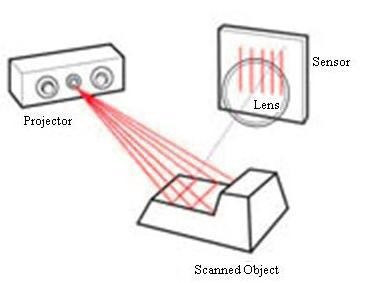
\includegraphics[width=.9\linewidth]{images/structured-light-scan}
	  \caption{}
	\end{subfigure}%
	\begin{subfigure}[b]{.33\textwidth}
	  \centering
	  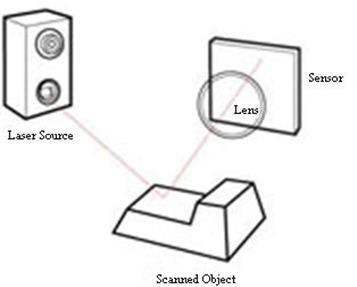
\includegraphics[width=.9\linewidth]{images/triangulate-laser-scan}
	  \caption{}
	\end{subfigure}
	\begin{subfigure}[b]{.33\textwidth}
	  \centering
		\begin{tikzpicture}[scale=2.5]

		\coordinate [label={[black]above:$Source$}] (A) at (0, 1);
		\coordinate [label={[black]above:$Sensor$}] (B) at (1, 1);
		\coordinate [label={[black]below:$Object$}] (C) at (0.5, 0);

		\draw[green] (A) -- node [above] {$c$} (B);
		\draw[black] (B) -- node [right] {$ $} (C);
		\draw[red] (C) -- node [left] {$b$} (A);

		\tkzMarkAngle[fill=white, size=0.25cm,%
		opacity=1](C,A,B)
		\tkzLabelAngle[pos=0.15](C,A,B){$\color{blue}A$}

		\tkzMarkAngle[fill=white,size=0.25cm,%
		opacity=1](A,B,C)
		\tkzLabelAngle[pos=-0.15](C,B,A){$\color{orange}B$}

		% \tkzMarkAngle[fill=green,size=0.25cm,%
		% opacity=.4](B,C,A)
		% \tkzLabelAngle[pos= 0.15](B,C,A){$ $}

		\end{tikzpicture}
		\caption{}
	\end{subfigure}
	\caption{Triangulation 3D scanners \protect\footnotemark}
	\label{fig:triangulation-scanners}
\end{figure}

Given the precise distance between the light source and sensor ($\begingroup\color{green}c\endgroup$) and as well as the outgoing angle of emitted light ($\begingroup\color{blue}A\endgroup$) and incoming angle of reflected light ($\begingroup\color{orange}B\endgroup$), the distance to the object is given by $\begingroup\color{red}b\endgroup = \begingroup\color{green}c\endgroup\frac{ sin(\begingroup\color{orange}B\endgroup)}{sin(\pi - \begingroup\color{blue}A\endgroup-\begingroup\color{orange}B\endgroup)}$.

\subsection{Time of flight scanners (TOF)} \label{subsec:tof}

\begin{figure}[ht]
  \centering
  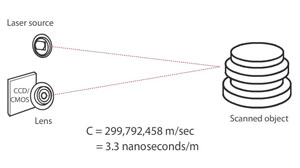
\includegraphics[width=.5\linewidth]{images/pulse-tof}
  \caption[Time of flight scanner]{Time of flight scanner \protect\footnotemark}
  \label{fig:tof}
\end{figure}
\footnotetext{Source: \url{http://www.rapidform.com/3d-scanners/}}

Time of flight (TOF) scanners emit laser pulses just like triangulation laser scanners. Unlike triangulation scanners, time of light scanners measure the time taken by a pulse to reflect to be detected by the scanner's sensor (see \autoref{fig:tof}). The distance travelled by the pulse can be computed by considering the speed of light. Given the time it takes for a pulse to travel to a surface and back to the scanner ($t$), the distance ($d$) is given by $d = ct/2$ where $c$ is the speed of light. The accuracy of the distance calculation depends on how precisely time can be measured \cite{Form2014}.

\begin{figure}[ht]
	\begin{tikzpicture}[scale=1]
	\begin{axis}[
		width=1\textwidth,
		height=150,
	    axis lines = left,
	    yticklabels={,,},
	    xticklabels={,,},
	    axis x line=center,
	    xlabel = $Time$,
	    ylabel = {Amplitude},
	    legend style={
	    at={(1,0)},
	    anchor=south east}]
	]
	\addplot[samples=500,domain=0:2*pi, color=red]{sin(deg(x))};
	\addlegendentry{Transmitted signal}
	\addplot[samples=500,domain=0:2*pi, color=blue]{sin(deg(x-pi/2))};
	\addlegendentry{Received signal}
	\draw[<->] (axis cs:2.61799,0.5) -- node[above]{Phase shift $t$} (axis cs:4.18879,0.5);
	\end{axis}
	\end{tikzpicture}
	\caption{Phase shift in returned signal}
	\label{fig:phase-shift}
\end{figure}

Laser phase-shift scanners \cite{Frohlich2004} are a variation on the standard TOF scanner. These scanners modulate the power of the laser pulse in a sinusoidal wave during a scan. The phase shift in the returning pulse is then used to compute the round trip time (see \autoref{fig:phase-shift}). Due to the cyclical nature of the signal, phase shift is ambiguous. This ambiguity is resolved by using measurements at multiple frequencies \cite{Bhurtha}.


\subsection{Comparison}

Laser and structured light triangulation scanners can achieve 10 micrometer accuracy over distances less than one meter. Over longer distances, however, the triangle in \autoref{fig:triangulation-scanners} becomes elongated which results in more variance in the distance calculation \cite{Mackinnon2006} when compared to TOF scanners. Structured light scanners specifically are less prone to motion distortions when compared to laser scanners and tend to also be faster \cite{Brown2012}. Hand-held scanners triangulation are easy to set-up and use compared to other scanners. Accuracy, speed over short distances in combined with their low cost and portability make these scanners preferable for objects that can be scanned at short range.

The accuracy of TOF scanners is a function of how accurately a laser pulse round trip time can be measured. TOF scanners tend to be less accurate over short distances (typically less than 2 meters) as there is less distance over which to amortize measurement error. Larger distances up to 1 km can however be measured with high accuracy \cite{Form2014}. The speed of TOF scanners depends on the resolution required. Tens of thousands of points may take seconds while resolutions with millions of points may take minutes.

Phase-based scanners have a more limited range due to the cyclic nature of the sinusoidal pulse \cite{Bhurtha}. Objects from beyond the scanner's designed range can sometimes be erroneously interpreted as being far closer when the scanner fails to disambiguate pulses. Phase based scanners compensate for this disadvantage by being much faster and more accurate than traditional TOF scanners within a shorter range (2-100m) \cite{Form2014}.


\begin{table}
\begin{tabular}{ |l|l|l|l|l|l| }
  \hline
  Type &              Range &        Precision       & Speed & Portability \\
  \hline
  Structured light &    <1m     & 10 micrometer  & Seconds & High \\
  Laser triangulation & <1m     & 10 micrometer  & Seconds  & Medium \\     
  TOF &                 2-1000m & Medium      & Minutes & Low \\
  Phase &               2-100m & Low         & Seconds to Minutes & Low \\
  \hline  
\end{tabular}
\caption{Comparison of scanning technology}
\end{table}


\subsection{Range images} \label{sec:data}

\footnotetext{Source: \url{http://www.rapidform.com/3d-scanners/}}

\begin{figure}[ht]
  \centering
  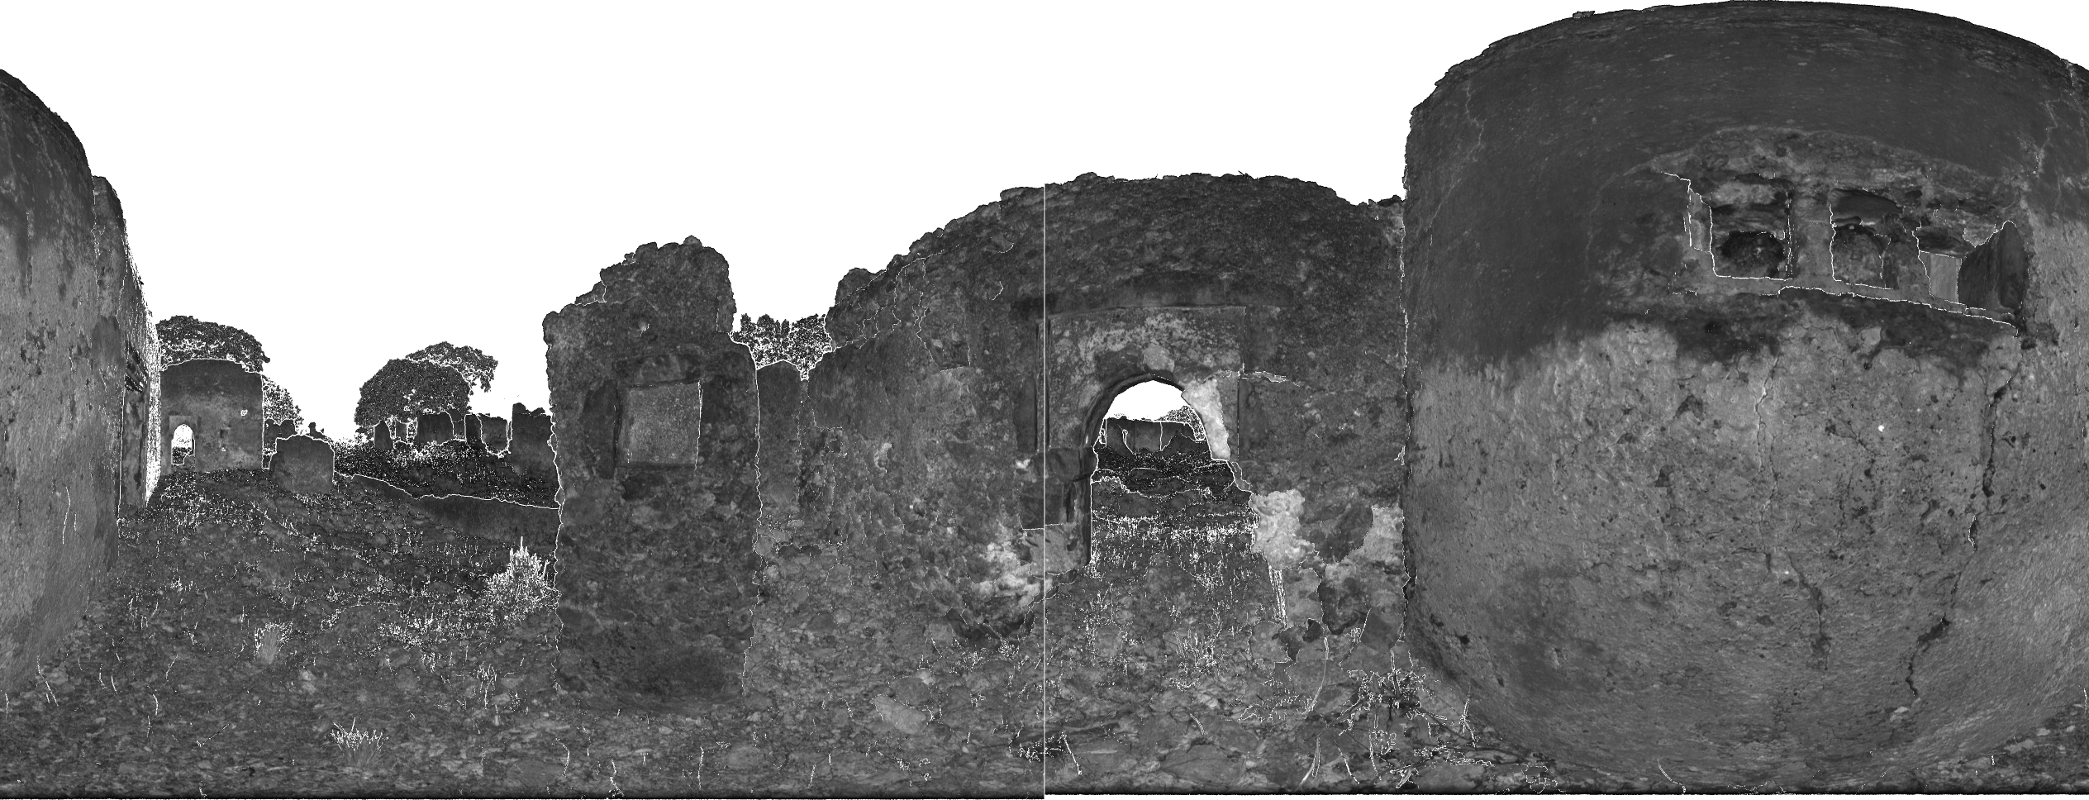
\includegraphics[width=1\linewidth]{images/grid}
  \caption{2D scan grid of intensity values \protect\footnotemark}
  \label{fig:grid}
\end{figure}

\footnotetext{Rendering based on data provided by the \href{http://www.zamaniproject.org/}{Zamani Project}}

The terrestrial laser scanner technology described above produces angle and range measurements that are converted into 3D coordinates relative to the scanner and returned as a range image. A range image is a two dimensional array of samples, that in addition to 3D coordinates, may also include the intensity of the returned laser pulse, as well as colour measurements, and other information specific to a scanner or manufacturer \cite{Frohlich2004}. We limit our investigation to range images produced by TOF and phase scanners that return an intensity value in addition to coordinates with every point. We exclude colour information as such scans were not readily available to us at the time of writing.

A range image is considered to be 2.5D rather than full 3D as it is limited to representing objects captured from a single perspective. When viewed in 3D, a range scan will contain many occluded objects. One will also notice the sampled point density reduces as one moves away from the scan origin. This can make it hard to identify objects in far away low density regions of a range image. Rendering a range scan as a grey scale 2D panoramic image (see \autoref{fig:grid}) may make objects more recognizable. The grid structure of range scans can also facilitate cheap neighbour searches (discussed later).

\section{3D reconstruction pipeline} \label{sec:pipeline}

% \todo{Used many of the same refs, find some others}

\begin{figure}

	% Define block styles
	\tikzstyle{decision} = [diamond, draw, fill=blue!20, 
	    text width=4.5em, text badly centered, node distance=3cm, inner sep=0pt]
	\tikzstyle{block} = [rectangle, draw, fill=gray!20, 
	    text width=5em, text centered, rounded corners, minimum height=4em]
	\tikzstyle{optionalblock} = [rectangle, draw, dashed,
	    text width=5em, text centered, rounded corners, minimum height=4em]
	\tikzstyle{line} = [draw, -latex']
	\tikzstyle{cloud} = [draw, ellipse,fill=red!20, node distance=3cm,
	    minimum height=2em]
	
	\centering

	\begin{tikzpicture}[node distance = 2cm, auto]
	    % Place nodes
	    \node [block] (acquire) {Scan acquisition};

	    \node [optionalblock, below right of=acquire, node distance=3cm] (clean) {\bf{Clean}};
	    \node [block, below left of=acquire, node distance=3cm] (register) {Register};
	    \node [block, below of=acquire, node distance=4cm] (reconstruct) {Reconstruct surface};
	    \node [optionalblock, right of=reconstruct, node distance=3cm] (autofill) {Automatic hole filling};
	    \node [optionalblock, left of=reconstruct, node distance=3cm] (filling) {Manual hole filling};
	    \node [block, below of=reconstruct, node distance=2cm] (texture) {Texture};
	    % Draw edges
	    \path [line] (acquire) -- (clean);
	    \path [line] (acquire) -- (register);
	    \path [line][<->] (clean) -- (register);
	    \path [line] (register) -- (reconstruct);
	    \path [line][-] (reconstruct) -- (autofill);
	    \path [line] (reconstruct) -- (filling);
	    \path [line] (filling) -- (texture);
	    \path [line] (reconstruct) -- (texture);

	    \draw[densely dotted] (1.7,-5.3) rectangle (4.7,-6.7);

	    % legend
	    \node [block, right of=texture, node distance=2.5cm, scale=0.7,
	    	text width=3.8em, minimum height=1em](required) {Required step};
	    \node [optionalblock, right of=required, node distance=1.4cm, scale=0.7,
	    	text width=3.8em, minimum height=1em] (notrequired) {Optional step};

	\end{tikzpicture}

	\caption{Reconstruction pipeline \protect\footnotemark}
	\label{fig:pipeline}

\end{figure}
\footnotetext{Adapted from \citet{Ruther2011}}

3D reconstruction of a site starts with the acquisition of range scans in the field. The collection of raw scans are then subjected to a series of processing steps. Unwanted objects and noise are typically removed and missing data can be synthesized. The scans are then transformed into a common coordinate frame in a process called registration. A surface model can then be constructed from the registered point sets. The final model is complete when the reconstructed mesh is textured (see \autoref{fig:pipeline}) \cite{Ruther2011}.

\subsection{Data acquisition}
Some degree of planning is required to ensure the successful 3D acquisition of a heritage site. One needs to decide on an appropriate level of scan detail, as the set resolution of a scanner determines the data acquisition rate. Scanner positions that result in flat angles of incidence with surfaces should be avoided to maximize sample density and surface detail. Good scanning positions will ensure that maximum site coverage is achieved in the most economical way.

Additional considerations can speed up later steps in the pipeline. Automated registration tools require that that overlap between scans is achieved. Ensuring that the scanner is consistently at the same level and orientation can simplify registration \cite{Ruther2011}.

\subsection{Registration}  \label{sec:registration}

\begin{figure}[ht]
  \centering
  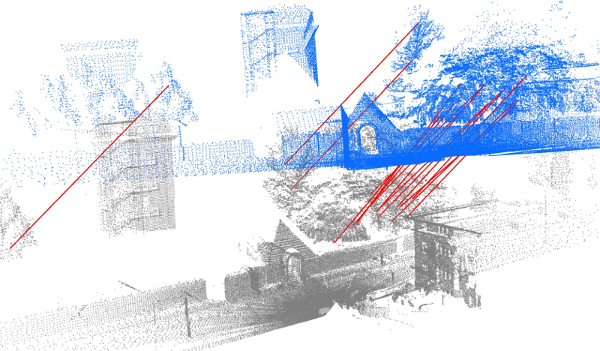
\includegraphics[width=0.6\linewidth]{images/registration}
  \caption{ICP correspondences \protect\footnotemark.}
  \label{fig:registration}
\end{figure}
\footnotetext{Source: \url{http://pointclouds.org/documentation/}}

Two approaches are commonly used to transform all scans into a common coordinate system. The first approach requires placing reference objects, called targets, around a site during data acquisition. When the same object is found in two scans, the object's target can be used to align the scans \cite{Besl1992}. The second approach, Iterated Closest Point (ICP) aligns scans by using surface features \cite{Bernardini2002}.

Automated systems easily identify targets and provide highly accurate registration. Targets do, however, have to be captured in high resolution in order to be useful. This may require one to capture more scans than required for simple documentation purposes. In the heritage domain, targets have been found to be impractical as they often need to be placed in hard to reach places and intricate indoor environments require too many targets \cite{Ruther2011}.

ICP requires less effort during data acquisition. However the registration procedure requires that two surfaces are roughly aligned as an initial condition, usually by hand. Correspondences are then computed between the surfaces and an incremental transformation is then computed to minimize the distance between all the correspondences. After the transformation is applied, the procedure is repeated until convergence is reached \cite{Rusinkiewicz}. There are many versions to the ICP algorithm that vary mainly in the type of correspondent matching and optimization procedure used.

A user needs to ensure a good initial alignment or convergence may not be achieved. Featureless surfaces are also problematic as the optimization problem will have multiple solutions which may lead to misalignment.

\subsection{Cleaning}\label{sec:cleaning}

\begin{figure}[ht]
	\begin{subfigure}[b]{.5\textwidth}
	  \centering
	  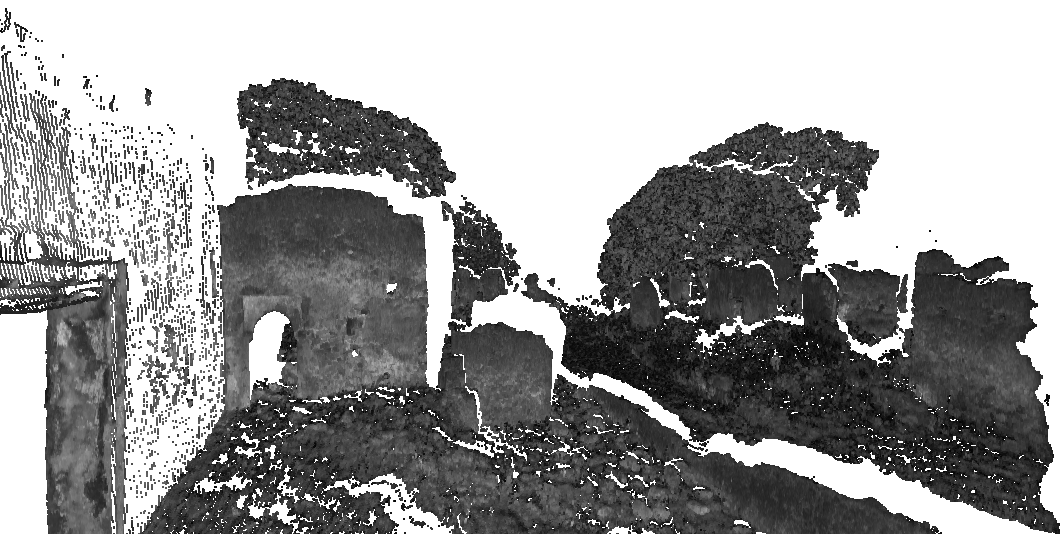
\includegraphics[width=.9\linewidth]{images/dirty}
	  % \caption{Structured light 3D scanning \cite{Form2014}}
	  % \label{fig:structured-light-scan}
	\end{subfigure}%
	\begin{subfigure}[b]{.5\textwidth}
	  \centering
	  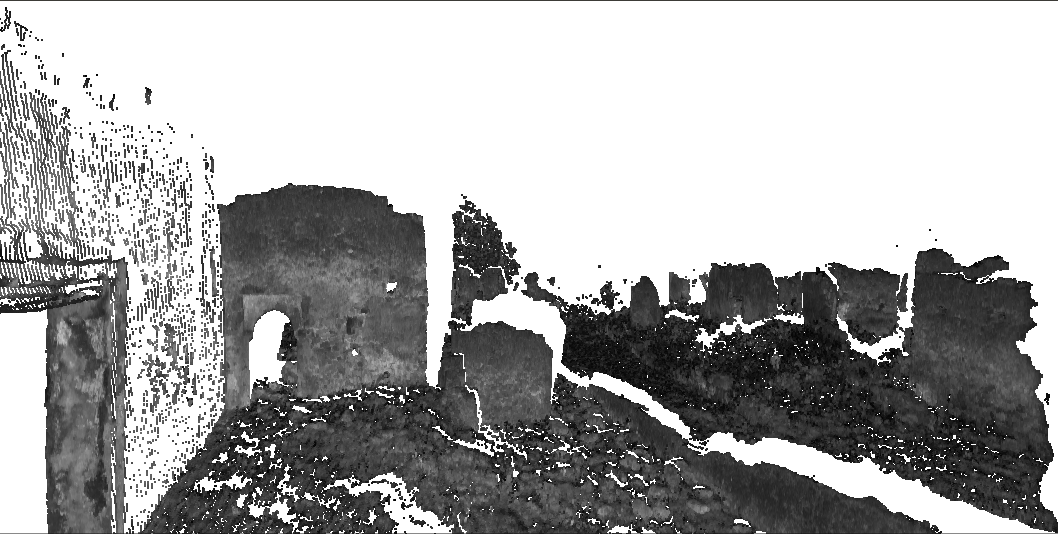
\includegraphics[width=.9\linewidth]{images/clean}
	  % \caption{Laser 3D scanning}
	  % \label{fig:images/triangulate-laser-scan}
	\end{subfigure}
  \caption{Trees cleaned from a scan}
  \label{fig:cleaning}
\end{figure}

Cleaning is considered an optional step for documentation purposes. However, skipping it in the modelling pipeline can lead to poor results during surface reconstruction (see Section \ref{sec:reconstruction}). The aim of cleaning is to remove trees, people, cables, cars, doors, animals and other unwanted objects, as well as scanner artefacts.

An object is usually removed either because it is not part of the subject matter or it won't mesh well later in the pipeline. Cars parked near monuments or power lines are frequently removed. Trees or other vegetation may be considered as part of the subject matter but are often removed because meshing algorithms do not produce good results when they are present.

Artefacts are unwanted points that result from of imperfect equipment rather than physical surfaces. Distant samples that are interpreted as being close by in phase-based TOF scanners are one such instance (see Section \ref{subsec:tof}). Incorrectly binned points will appear normal in a 2d rendering but will look like noise in 3D. The sun or other light sources can also result in artefacts. Noisy artefacts can also be the result of fog or smoke in an environment \cite{Ruther2011}.

% \todo[inline]{More detail on artifacts}

\begin{figure}[ht]
  \centering
  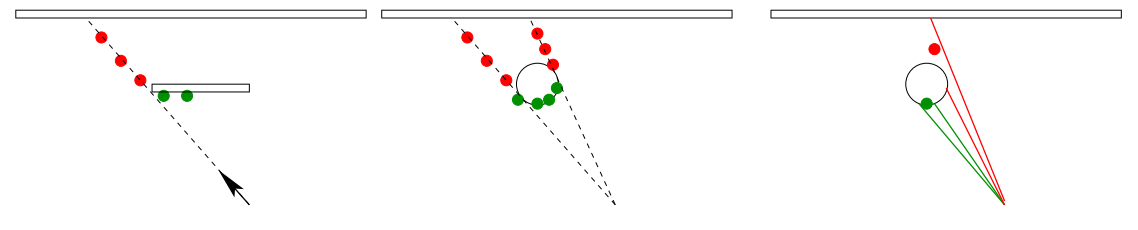
\includegraphics[width=1\linewidth]{images/mixed-pixel}
  \caption{Mixed pixels. Green are valid points and red are not. \cite{Tuley2005}}
  \label{fig:mixed-pixel}
\end{figure}

Mixed pixels is phenomenon that can occur when a laser pulse partially strikes a nearby and distant object. The result is an interpolated data point between the near and far object \cite{Tuley2005} (see \autoref{fig:mixed-pixel}). This typically manifests as column of points behind doorways or close to other edges. \\

Cleaning scan data is typically a manual task requiring expert judgement. It can be performed on individual scans before registration or after registration \cite{Ruther2011}.

Cleaning single scans before registration typically requires less system resources as less data needs to be loaded. Loading multiple large scans can be problematic on less capable hardware. One may, however, choose not to remove all unwanted objects as some objects may necessary for registration. A tree on a flat surface may be necessary for correspondence matching in ICP. Without these objects automated registration may not converge on feature-sparse surfaces. Registration and cleaning may thus, in practice, be an iterative process. Removing objects from the registered set of range images may be easier due to the following. An increased number of samples from multiple perspectives can make objects easier to recognize. It may also be possible to remove an unwanted set of points from multiple scans in one action. System resource constraints can be managed by loading one or more scans at a time.

After registration, all range images are combined into a single large point cloud. The combined dataset is typically too large to fit into memory and few software packages can support data sets of this size. It is possible to clean the combined point cloud by loading slices. When doing so one does not have the benefit of referencing the 2D range image when cleaning the combined data set. One would also have trouble mapping the result back to the original scans for archival purposes. The 2D array structure of range images also supports performing constant neighbour lookups. If this is not done $O(log(n))$ octrees or kd-trees will be necessary which can slow down feature computations.

Some large heritage scanning projects have reported typical scans taking from 30 minutes up to 120 minutes to clean by an experienced person \cite{Ruther2011}. High resolution scans can take up to a full day to clean. Existing tools leave much to be desired in terms of cleaning efficiency. More detail is presented in section \ref{sec:interactive-tools}.

\subsection{Surface reconstruction}  \label{sec:reconstruction}

% \begin{figure}[ht]
%   \centering
%   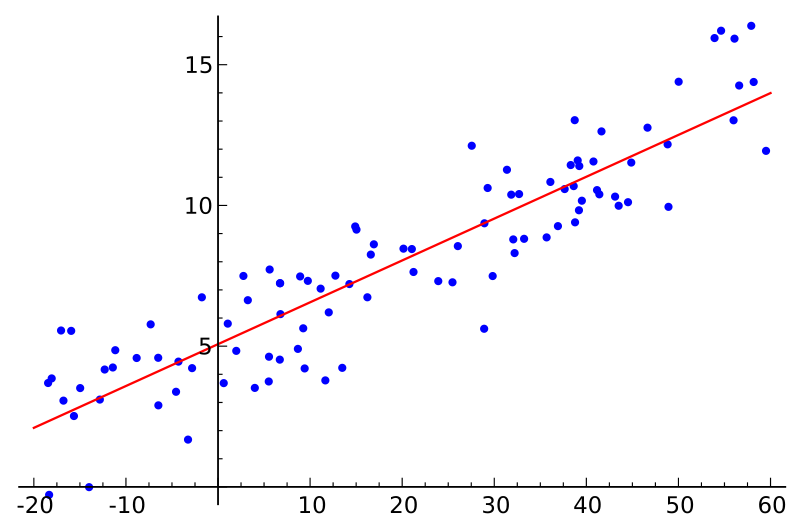
\includegraphics[width=0.6\linewidth]{images/mls}
%   \caption{Surface fitting \protect\footnotemark.}
%   \label{fig:registration}
% \end{figure}
% \footnotetext{Source: \url{http://en.wikipedia.org/wiki/File:Linear_regression.svg}}

Surface reconstruction converts the discrete point model into a triangulated surface model. This can be achieved either via interpolation methods, that aim to connect neighbouring points by computing a triangulation, or by approximation methods that aim to approximate a surface that fits the samples \cite{Schall2005}.

Interpolation methods are very sensitive to noise. Poor triangulations are achieved when scans are not properly registered or the sampling exhibits high variance. A preprocessing step can mitigate these problems but tends to be time consuming and often leads to a loss of detail \cite{Ruther2011}.

Surface approximation algorithms are less susceptible to noise. Poisson surface reconstruction \cite{Kazhdan2006} is a popular method that is noise resistant and achieves great detail. It uses samples with normals to interpolate a normal field and then solves a Poisson equation to compute an indicator function. Results are dependent on good normal estimations. It is thus preferable to compute normals prior to registration when using this approach. Poisson surface reconstruction produces ``water-tight'' surfaces and automatically fills small holes. While this is useful for producing a visually pleasing 3D model, it does not result in a historically accurate model because new surface data may be synthesized in the process.

Moving Least Squares (MLS) is another popular surface approximation method that does not over smooth and interpolate missing data \cite{Alexa2003}. Like Poisson, it also requires normal estimates. MLS computes a local surface approximation at a sample point by considering its neighbourhood. Every point in a neighbourhood is weighed according to its importance. A surface is then computed by minimizing the weighed distance to the surface for each point in the neighbourhood. Poisson and MLS have both been adapted for out-of-core execution and GPU acceleration \cite{Merry2014}. \todo{Discuss issues else it may look perfect}\\


\subsection{Hole filling} \label{sec:filling}

It is unlikely that a scanning expedition will achieve complete coverage of a site. Furthermore, points are removed during cleaning and reconstruction of the surface. Hole filling is an optional step in the reconstruction pipeline that seeks to synthesize missing data \cite{Sharf2004} \todo{Expand}. For historical accuracy, hole filling is not desirable as data is synthesized. However, models that have been filled are more aesthetically pleasing. If holes are filled it is thus important to know what data has been synthesized.

Small holes can be filled automatically by surface reconstruction algorithms (in discussed in \ref{sec:reconstruction}). Larger patches are harder to fill convincingly with automated methods and may require manual effort to produce good results \cite{Ruther2011}.


\subsection{Texturing} \label{sec:texturing}

The final, but optional, step of the reconstruction pipeline is texturing. Colour in a model is not only visually pleasing but also form part of the historical record. Some laser scanners are equipped with cameras to capture colour information for each sample. Although this is very convenient, some in the heritage community have reported that poor texturing is achieved when compared to external cameras \cite{Ruther2011}. The biggest problem when texturing a model is dealing with different light conditions during the day. Capturing photos around the same time of day across multiple days is one way to mitigate the problem.

A model is textured from a series of photos by projecting the images onto the model. In order to achieve this, internal and external camera parameters needs to be known from time the picture is taken. This includes the position and orientation of the camera as well as the focal length of the lens. If this is not known it can be estimated via software by selecting or computing correspondences between pictures \cite{Ruther2011}.

% \todo{more citations on texturing, ask rudy}


\section{The cleaning problem}

In the previous section the point cloud cleaning task was framed in the context of the 3D reconstruction pipeline. In order to set clear goals it is important understand what point cloud cleaning entails.

% In this section we will look at the current state of point cloud segmentation tools and frame the point cloud segmentation problem.

% In the previous section 3D reconstruction from laser scans in a heritage preservation context was discussed. Environmental and instrument noise in laser scans are hard to remove and can be taxing in terms of human resources. The goal of this research is to speed up the cleaning process through tools and semi automated methods. Given the noise characteristics and properties of the point cloud data sets made available the problem is outlined below.


\subsection{Tools}

\begin{table*}[htb]
\centering
  \begin{tabular}{| l | x{3cm} | x{3cm} | c |}
	\hline & Interactive tools & Filters & Open source \\    
    \hline
	
		Terrascan \cite{Terrasolid2012} &
		&
		ground points, vegetation, buildings &
		\tickNo \\

	\hline
		Pointools Edit \cite{Pointools2012} &
		lasso select, rectangle select, ball and cube brush select, floodfill with distance threshold, floodfill based on colour or intensity similarity, plane select &
		&
		\tickNo \\
	
	\hline
		VR Mesh Studio \cite{VirtualGrid2012} &
		power lines &
		ground, vegetation, roofs, planes &
		\tickNo \\
	
	\hline
		Carlson PointCloud \cite{Carlson2012} &
		&
		clear isolated and duplicate points, extract bare earth &
		\tickNo \\
	
	\hline
		3D Reshaper \cite{Technodigit2012} &
		lasso select &
		clustering with distance metric, clustering colors, remove isolated points &
		\tickNo \\
	
	\hline
		Cyclone \cite{Leica2012} &
		lasso select, floodfill based on smoothness similarity &
		&
		\tickNo \\
	\hline	
		Meshlab \cite{VisualComputingLaboratory2012} &
		point picking, plane select &
		isolated point removal &
		\tickYes \\
	\hline	
		Cloud Compare &
		point picking, polygon select, rectangle select &
		&
		\tickYes \\
	\hline
  \end{tabular}
  \caption{Existing systems}
  \label{table:software}
\end{table*}


% As efficiency of a tool increases the accuracy  


% Object recognition is a difficult computer vision problem that humans can often solve instantly. State of the art vision algorithms can be computationally expensive and need to be trained to perform recognition tasks. 

% The problem can be approached by a human or machine.

% The distinction between wanted and unwanted points is somewhat subjective and dependent on one's interpretation of the data. Object recognition is an essential part 

% is to group points according to their properties. At a very high 

% An ideal solution would be a fully automated and require no human interaction. It is however sometimes difficult, even for humans, to unambiguously determine whether a point is part of an important structure or simply noise. Different people may segment the same scene differently. It is unlikely that an automated solution would be satisfactory in all cases due a large degree of classification subjectivity between people. \todo{Cite a hard problem in vision to justify this?}\\

% We will not attempt a fully automated solution to the problem but rather frame it as an interactive segmentation problem. The user is thus at the center of the cleaning process. The goal is to provide a set of tools that will speed up or automate parts of the task while maintaining accuracy.


Point cloud cleaning is in essence a segmentation problem. The high level goal is to divide a point set into wanted and unwanted points. In order to make this distinction it is important to recognize what points in a scene represent. Humans are very good at object recognition which is part of the reason why point cloud cleaning has remained a very manual task. Despite this general proficiency, software interfaces often make it hard to group points according to their perceived class.

In order to facilitate efficient point cloud cleaning, or general point cloud editing, software packages provide a range of tools. Tools that do more tend to perform tasks less accurately. In order to be effective, a system should provide tools with both large and small areas of influence so that crude segmentations may be refined and the desired accuracy be obtained with minimal effort. In lieu of a fully automated solution it is also important that tools be computationally efficient so that interactivity is maintained.


% The most accurate tool would let a user label a single point at a time. At this level of accuracy it might take a long time to complete a segmentation task. On the opposite side of the spectrum, a tool could automatically label all points. This could maximize efficiency but would likely not be very accurate as object recognition is a difficult computer vision problem.  State of the art vision algorithms can be computationally expensive and need to be trained to perform recognition tasks.




% When offloading part of the segmentation task to semi-automated tools, it is important to allow the user refine the result. It is thus necessary to provide more accurate manual tools to correct possible mistakes. Because the user is expected to refine semi automated segmentations, it is important for semi automated tools to be fast.

A number of open source and commercial software point cloud packages are available (see \ref{table:software}). As the source code and technical descriptions of proprietary packages are not available, they will be treated as black boxes. The software packages surveyed contain two types of tools which we shall refer to as interactive tools and filter tools. Interactive tools provide immediate feedback and are driven primarily via mouse and keyboard input. Filter tools on the other hand are controlled via parameters and operate a set of points that are specified prior to use.

\subsubsection{Interactive tools}\label{sec:interactive-tools}

The most basic interactive tool is \emph{point picking} which allows one to select a single point. It is not very effective for cleaning purposes. \emph{Meshlab} \cite{Cignoni2008}, an open source mesh manipulation program, includes this tool. It is more likely to be useful when editing meshes.

The \emph{polygon select} tool is one of the more useful interactive tools. The tool lets the user select points by constructing a 2D polygon around a set of points on the view port. It is useful when selecting points that are isolated in space. Polygon selection becomes problematic when one is unable find a perspective that separates the target points from its neighbours. \emph{Cyclone} is a proprietary package \cite{Leica2012} that solves this problem by restricting the tools area of influence with a limit box. Cyclone also allows a user TO pan the view port while constructing a polygon. Meshlab has a similar tool that is limited to rectangular areas. \emph{Cloud Compare} \cite{CloudCompare} is another open source package that provides both a polygon and rectangular select version of the tool.

\emph{Brush tools} are another class of interactive tools that lets one select points by painting on the view port. The `brush' shape is typically a sphere but packages like \emph{Pointools Edit} \cite{Pointools2012} also provide additional shapes such as a cube. Brush tools has the same disadvantage as the polygon select tool when it comes to selecting points that cannot be isolated via perspective.

\todo{State that we overcome this by only operating on layers}

\begin{figure}[ht]
  \centering
  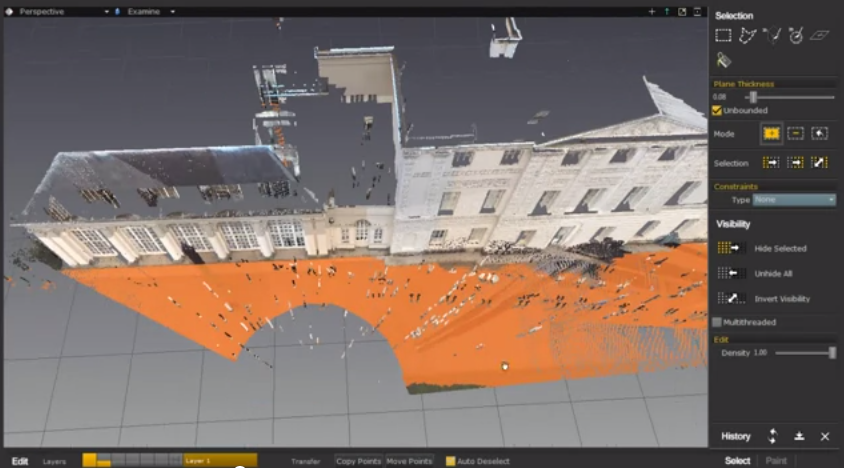
\includegraphics[width=1\linewidth]{images/plane}
  \caption{Plane selection tool in Pointools \cite{Pointools2012}}
  \label{fig:plane-select}
\end{figure}

Interactive \emph{flood fill} tools not unlike those found in raster image editors are also common in point cloud packages. The tool labels points by growing a region from a user selected seed point. Various membership criteria can be specified in order to limit the selection. Pointools \cite{Pointools2012} allows a user to restrict the selection by specifying a threshold in terms of colour or intensity value. Pointools as well as Meshlab includes a variation that selects planes (see \autoref{fig:plane-select}). Cyclone \cite{Leica2012} provides a smoothness constraint that lets one select regular surfaces. More specialized flood fill tools can perform power line removal, such as the tool found in \emph{VR Mesh Studio} \cite{VirtualGrid2012}. The success of a flood fill tool depends on good threshold being set. If the user is responsible for specifying these values it may be hard to use for less sophisticated users. Meshlab uses a novel technique that allows a user to limit the extent of the flood fill by dynamically controlling a threshold via the mouse wheel. This is used in both the Meshlab plane selection tool and the vertex clustering tool (which uses the distance from the original selection as a threshold).

\subsubsection{Filters} \label{section:filters}

Filters can range from simple denoising functions to complex machine learning algorithms. Software packages generally allows one to restrict a filter's area of influence.

Meshlab provides a number of denoising filters. \emph{Outlier removal} allows a user to specify the number of neighbours a point is required to have in order to not be removed. This tool is problematic when used with range images due to the decreasing point density away from the scan origin. Points close to the origin are less likely to be classified as outliers due to the higher point density while false positives are more common further away where there are fewer samples.

\begin{figure}[ht]
  \centering
  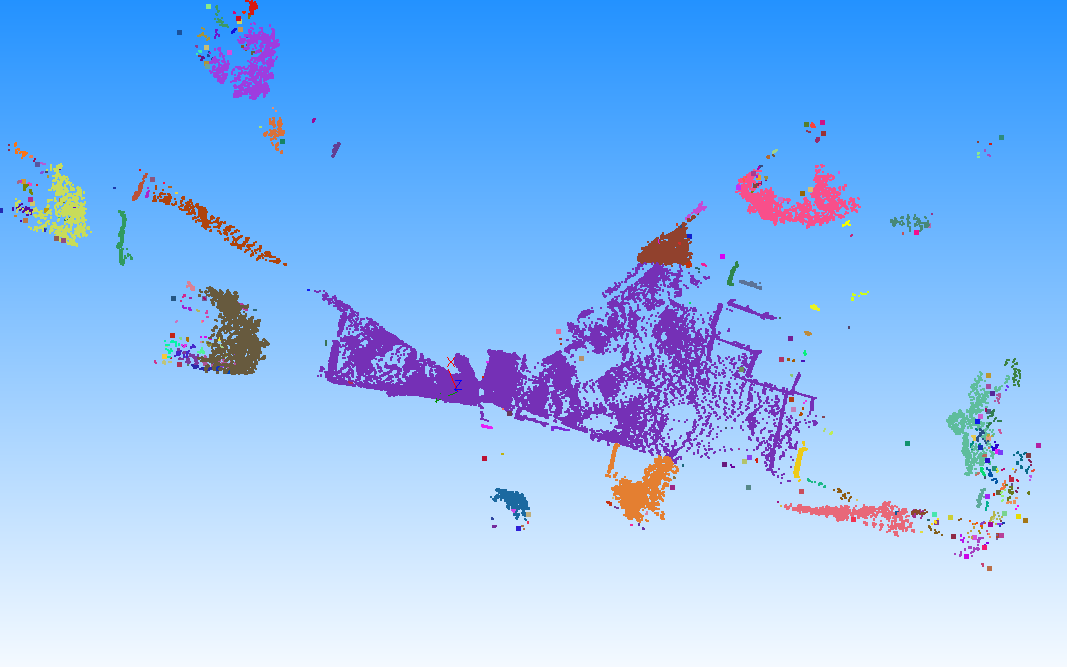
\includegraphics[width=1\linewidth]{images/clustering}
  \caption{Clustering issue in 3D Reshaper \cite{Technodigit2012}}
  \label{fig:clustering-issue}
\end{figure}

\emph{Clustering} tools are also affected by non uniform density. \emph{3D Reshaper} \cite{Technodigit2012} provides a filter that groups spatially related points. This approach work fine on uniform point clouds. However, range scans poses a problem as more clusters are detected further away from the origin (see \autoref{fig:clustering-issue}).

\begin{figure}[ht]
  \centering
  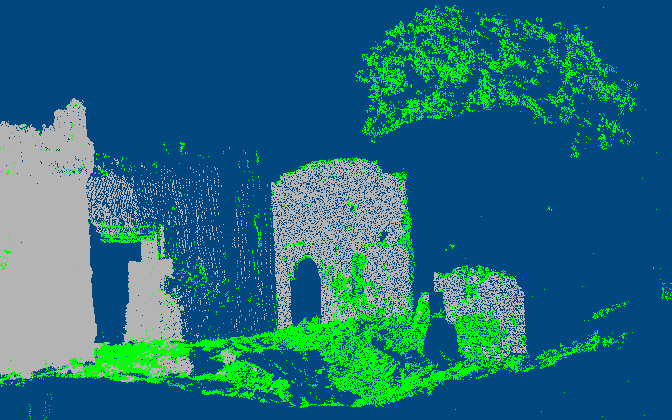
\includegraphics[width=1\linewidth]{images/vrmesh-veg}
  \caption{Vegetation filter in VR Mesh Studio \cite{VirtualGrid2012}}
  \label{fig:vegetation-issue}
\end{figure}


More specialized filtering tools exist, including ones aimed at extracting the ground plane \cite{Terrasolid2012, VirtualGrid2012}, finding rooftops \cite{VirtualGrid2012}, walls \cite{VirtualGrid2012}, buildings \cite{Terrasolid2012} and vegetation \cite{Terrasolid2012}. Most specialized filters are aimed at the surveying community who have different needs to those working in heritage domain. Eroded old structures are not easy to segment using tools designed to segment modern buildings that are more regular in shape. The heritage preservation community also has a strong emphasis on accuracy. Segmentations that may be satisfactory in other domains, such as surveying, may be far to crude for people  the heritage domain. Vegetation removal is one such instance. VR Mesh Studio's \cite{VirtualGrid2012} filter for segmenting vegetation detects plant growth on eroded ruin walls (see \autoref{fig:vegetation-issue}). False positives can be tolerated when searching for vegetation in a scene. It is is more problematic when the goal is to remove the identified points.

\subsection{Interface}
A user ultimately needs to judge whether a point is wanted or not. It is thus important for the system to present the data in a way that is easy to interpret and easy to interact with. Failing to do so will make cleaning more difficult.

Meshlab and Cloud Compare violate the important usability heuristic by not including an undo feature \cite{Nielsen2005}. Cleaning is a time consuming task and making a mistake can derail hours of work. The lack of an undo function can also slow a user down by requiring greater caution \cite{Miller1977}. Propriety packages tend to be more usable in this regard.


% Familiarity helps new users quickly get started. It is thus worth while looking at the interfaces of existing systems.
The tools surveyed all presented the user with an interactive 3D rendering of a point cloud. In addition to this Z+F \cite{Z+F2014} provides users with a 2D range image view. Humans are more adept at interpreting 2D data despite our environment being 3D \cite{Livingstone1987}. In order to perceive depth on a screen, an object has to move \todo{Cite, move or stereo vision, Patrick: depth cues}. Given that a range scan does not reveal more information as one's 3D perspective shifts, it is questionable whether a 3D view is best suited for range scan segmentation. \note{Depth aware fill fixes this for 2D}\\

Interfaces typically provide two ways to navigate a 3D scene. One can either transform the point cloud (object centric navigation), or manipulate the camera (camera centric navigation). All systems surveyed implemented object centric navigation. Cloud Compare and Meshlab amongst others render a track ball around the center of rotation. This makes it easier to reason about the interaction, especially when the center of mass is not at the scan origin. Cloud Compare and other systems lets a user set the center of rotation. In Meshlab, the center of rotation is fixed at the coordinate system origin. Object centric navigation is more intuitive when viewing movable objects. Environments however, are typically viewed from an upright perspective. Moving in and around a 3D environment from a 1st person perspective is more natural than moving the environment around. A rotated heritage site is not a familiar perspective and is likely to disorient a user.

Some systems use lighting when rendering the the point cloud. Meshlab lets one toggle lighting on and off. With lighting switched on the interface becomes less responsive when viewing large data sets. Lighting may help interpret a scene when viewing point clouds with no intensity or color information. However, when this information is available, such as with our data sets, it is questionable whether any value is added as artificial lighting may conflict with shadows captured at the time of the scan.


\section{Summary}
In this chapter a high level overview of digital the heritage preservation process was presented. Removing instrument noise and unwanted objects from range scans is a difficult and time consuming part thereof. Existing software packages provides a range of tools that aim to make point cloud manipulation easier. The tools that automate the segmentation of large regions, however, have issues dealing non uniform density range images and eroded heritage structures. Open source point cloud editing tools are few and are less capable than their propriety counterparts. Introducing equally or more advanced tools into open source frameworks may improve user productivity. However, systemic usability problems, such as the lack of undo, will hold users back. To address these issues, we introduce a newly created open source range image cleaning framework in the next chapter. This framework takes into account usability concerns and will provides a solid baseline on which to build the more effective cleaning we develop tools in later chapters.


% Terrestrial laser scanning is the primary tool used in digital heritage preservation for the documentation and 3d reconstruction. Triangulation scanners are more suited for scanning over short distances while TOF scanners work best for longer ranges. Traditional TOF scanners are slow but the phase based variation improves in speed while sacrificing range and potentially introducing noise.

% Only TOF scanners are considered in this research. The data set returned from a TOF scanner varies between manufacturers. Datasets used here are in a grid structure and contain X, Y, Z coordinates as well the intensity of the reflected laser pulse. Manufacturers may also associate color with each point as well as raw scan data.

% Laser scanner data sets need to be processed to create 3D models. This process includes cleaning, registration, meshing, hole filling and texturing.

% During cleaning there are two types of noise that needs to be removed: instrumentation noise created by the scanner and environmental noise that is created by physical objects in the scene. Scanner manufacturers typically provide software that semi automatically remove instrumentation noise with varying levels of success. Removing environmental noise however is typically a more manual endeavor. The cleaning task is a very time consuming part of the reconstruction pipeline.

% In this work we attempt to find ways to speed up the cleaning process through tooling and semi automated methods. We focus this on methods applicable to TOF scans in a grid form with X, Y, Z and intensity values.


% \subsubsection{Segmentation}

% In the sections above we presented a high level overview of the point cloud cleaning task and the tools available to complete it. We now approach segmentation from the bottom up and introduce the different types techniques we can apply to tackle separate wanted from unwanted points.

% The goal of segmentation is to partition a scene into meaningful subsets. There are many possible partitions for any range scan. To produce meaningful segments we need a model of what needs to be segmented based on prior world knowledge. 

% In some instances it may be simple segment to a scene by simply using raw data. If we made the observation that tree bark absorbs laser light more than other objects in a scene, we could use the intensity of the laser light captured by the scanner to segment local neighborhoods of tree bark. If we were trying to segment an entire tree instead of just the bark, it may be hard to express a model in terms of raw range scan data. Abstracting the data may make it easier to express a model. Feature extraction, clustering and classification are ways that can help us simplify the segmentation processes by creating higher level abstractions to work with.


% \subsubsection{Features}

% A feature is a loosely defined term used in many disciplines including statistics, machine learning and computer vision \cite{Flach2012}.
% Features are generally floating point or integer values but can also be categorical values.

% A feature is a numeric attribute that characterizes one or more samples in a image, range scan or more generally a dataset. Features are used many domains including statistics, machine learning and computer vision. Features can be designed to only describe characteristics pertinent to the task at hand and be invariant to extraneous variables \cite{Flach2012}. When analyzing images in computer vision it's desirable to have features that are invariant to lighting conditions and the orientation of the camera. Features without these properties are not very robust. 

% Unprocessed range scans describe positions of points in space, their relation to each other from the scanner perspective and the intensity of reflected light. The process of creating new descriptors from this data is called feature extraction \cite{Jain1999}. Point normals are one type of descriptor that can be extracted from range scans \cite{Klasing2009}. 

% Feature extraction is typically a preprocessing to a segmentation process. Because features are very useful in isolation, they are typically evaluated as part of a larger task \cite{Jain1999}.


% Data, information, knowledge


% From an information theoretic point we cannot create information.

% In computer vision features get rid of nuisances like lighting and transformations

% How to pick or generate good features
% 	Performance in an end to end task, together with a classifier and dataset

% 		it tells us nothing on how a given feature can be improved, or how performance generalizes to different classifiers and different data sets.

% Depends on the purpose

% Correspondences, scale invariant, orientation invariant


% \todo{Feature extraction, feature selection}

% Classification and grouping

% \subsubsection{Clustering}

% Cluster analysis is the organization data points into groups (clusters) based on similarity \cite{Jain1999}. Similarity is usually determined by grouping features into vector and comparing points via a distance metric in this multi dimensional space. Clustering is an instance of unsupervised learning in that the goal is to group unlabeled data into meaningful groups. The first step in a clustering algorithm is generally to select the most suitable features. Secondly a distance metric needs to be chosen in order to compare data points. Finally a grouping algorithm needs to be decided on. In order to efficiently represent clusters for further computation one may wish to extract a compact representation of the data. One could use the cluster centroid or compute a feature descriptor of the region. 


% Clustering divides things that are close into groups


% membership criteria and

% Euclidean distance is a common choice.

% and normalize them if necessary



% Clustering algorithms are hard to evaluate as 

% Validation


% Issues
% 	efficiency
% 	normalization


% Hard vs fuzzy partition

% Hierarchical clustering

% Graph theoretic clustering 
% 	Graph cuts
% 	Markov random fields

% Clustering is a useful ab


% \subsubsection{Classification}


% % Unsupervised
% % simulated annealing
% % feature extraction
% % HAVE NOT LOOKED AT SPLIT MERGE ALGORITHM



% Classification is the problem of determining what class ($Y$) an observation belongs to given a set of characteristics ($X$) \cite{Flach2012}. In our case this is determining whether an observed point in a range scan belongs to the wanted ($Y=wanted$) or unwanted ($Y=unwanted$) class given it's X Y Z and intensity values and relation to it's neighbors ($X$).

% While our ultimate goal is to classify a point as wanted or unwanted, it is easier to classify a point as belonging to one of a larger number of subclasses \cite{Malik2000}. For instance: trees, walls, person. The wanted/unwanted binary classification can then be expressed in terms of a point's membership to one of the intermediate classes. E.g. if a point belongs the tree class or person class, classify the point as unwanted, otherwise classify the point as wanted.

% %  There are many possible partitions of an image into subsets. There may not be a correct one. Bayesian view - there are many possible interpretations in the context of prior world knowledge. Some of this knowledge is low level such as coherence of brightness or color, equally important is mid to high level knowledge about symmetries of objects or object models. Partitioning is hierarchical image segmentation based on low level queues cannot and should not aim to produce a complete final correct segmentation \cite{Malik2000}

% % Segmentaion is the task of decomposing the dataset into constituent pastrts that have some higher level meaning

% % Unsupervised leaning is a good tool for silbing segmentation problem



% The characteristics used to determine the class of a point is also commonly referred as a feature \cite{Flach2012}. We will define a feature to be a piece of local information used in the classification task. The X Y Z \& intensity values of each point are the most elementary features in datasets we focus on. These features can be combined or processed to create derivative features. Point normals are examples of derivative features. Point normals are not present in our data set but can estimated by considering the positions of points in a local neighborhood \cite{Klasing2009}. Derivative features can simplify the classification problem by representing the data in a way that make it more meaningful and easier to relate a point to a class.

% A classifier is a model used to solve a classification problem. Classifiers can be divided onto two groups namely heuristic classifiers, and machine learning classifiers. Heuristic classifiers are constructed by encoding expert knowledge needed to solve a classification problem\cite{Clancey1985}. Machine learning algorithms construct a model from empirical data \cite{Flach2012}.

% Meshlab's denoising filter (see section \ref{section:filters}) is an example of a simple heuristic classifier. The classifier encodes the knowledge that a point is likely to be noise if it has less than $n$ neighbors within radius $r$. Heuristic classifiers can be very effective but are often hard to maintain and are not very flexible \cite{Flach2012}.

% Machine learning methods classify points by using patterns in the data that are often difficult for humans detect or encode. There are two main types of machine learning algorithms. Supervised learning algorithms infers a classification function from a labeled training dataset. Unsupervised learning algorithms attempt to uncover the hidden structure in a dataset without a training set \cite{Flach2012}.

% % Proprietary systems likely use some machine learning for more advanced classification filters. The vegetation filter in VR Mesh Studio \cite{VirtualGrid2012} could be achieved by training a supervised learning algorithm. The clustering filter in 3D Reshaper \cite{Technodigit2012} appears to an unsupervised learning algorithm such as k-nearest neighbors.

% % heuristic methods are not mutually exclusive with unsupervised leaning. Also called data mining.

% Then main disadvantage of supervised learning is that skilled workers are required to create labeled training sets. Training data needs to be representative of the types of data one wishes to classify. There is a large variety of unwanted objects and terrains one could encounter in a scanning expedition. Applying a supervised learning approach to point cloud classification could thus require a large upfront investment depending on types of objects one wishes classify and the types of environments one expects to encounter. The effectiveness of the resulting classifier would be largely dependent on how similar the training sets are to new data.

% Unsupervised learning algorithms differs from supervised learning in that it require no training data is used to construct a model. The model is created during classification task. The reduced human effort required aligns well with our goal of speeding up point cloud cleaning. Unsupervised learning however, cannot help us with applying a predefined set labeled to points. \todo{Clustering is related to image segmentation} Clustering can however help us too divide a dataset into groups of related points called clusters \cite{Flach2012}. How clusters are determined largely depends on what measure of relatedness is chosen. Unsupervised approaches are a good candidates for separating vegetation from structures.

% Semi supervised learning is another class of learning algorithms that falls between supervised and unsupervised. Semi supervised learning leverages small amounts of labeled data to construct an initial model. This model can then be refined using unlabeled data \cite{Flach2012}.

% Our goal to find the features that best correlate with the types of points that needs to be preserved or removed. While doing so we also aim to keep the computational cost low as to maintain an interactive cleaning work flow. Our goals are similar for creating classifiers from these features.

% \section{Summary}

% Terrestrial laser scanning is the primary tool used in digital heritage preservation for the documentation and 3d reconstruction. Triangulation scanners are more suited for scanning over short distances while TOF scanners work best for longer ranges. Traditional TOF scanners are slow but the phase based variation improves in speed while sacrificing range and potentially introducing noise.

% Only TOF scanners are considered in this research. The data set returned from a TOF scanner varies between manufacturers. Datasets used here are in a grid structure and contain X, Y, Z coordinates as well the intensity of the reflected laser pulse. Manufacturers may also associate color with each point as well as raw scan data.

% Laser scanner data sets need to be processed to create 3D models. This process includes cleaning, registration, meshing, hole filling and texturing.

% During cleaning there are two types of noise that needs to be removed: instrumentation noise created by the scanner and environmental noise that is created by physical objects in the scene. Scanner manufacturers typically provide software that semi automatically remove instrumentation noise with varying levels of success. Removing environmental noise however is typically a more manual endeavor. The cleaning task is a very time consuming part of the reconstruction pipeline.

% In this work we attempt to find ways to speed up the cleaning process through tooling and semi automated methods. We focus this on methods applicable to TOF scans in a grid form with X, Y, Z and intensity values.




% Machine learning
% Bayesian networks
% Statistical approaches
% Evolutionary approaches
% Neural nets

% Machine learning is a way of solving classification


% \begin{itemize}
% \item Point size
% \item Rendering depth vs intensity
% \item Navigation, fly through vs Track ball
% \item Exponential speed up in movement
% \end{itemize}


% \subsubsection*{CloudCompare}
% Supports colour clouds
% Rectangulkar, polygon select select tool
% Hide and show layers


% \subsubsection{Meshlab}
% Meshlab \cite{Cignoni2008} is the only viable open source tool we know of. It's primary purpose is mesh processing but it does allow one to work with point clouds through various plug-ins. Some plug-ins lets one preview an action but once it is applied it cannot be undone as Meshlab does not support undo. Meshlab supports opening multiple point clouds in the same view port but tools can generally only operate on one at a time.

% The viewport renders a track ball around the point cloud center at allows one to rotate it around its axis.



% \subsection{Set operations}
% Meshlab lets one invert selections

% \subsubsection{Z+F }

% \subsubsection{Point picking}
% Point picking is the most basic tool available to us

% \subsubsection{Lasso}
% Meshlab only rectangular

% \subsubsection{Brush tool}

% \subsubsection{Flood fill}

% \subsubsection{Plane selection}

% \subsubsection{Clustering}

% \subsubsection{Isolated point removal}

% \subsubsection{Limit box}



% \cite{Neisser1967}

% \subsection*{Summary}
% Semi automated tools
% Manual tools to correct imperfect results





% The user is the ultimate 

% For a user to classify a dataset. The software should let the user label wanted or unwanted points as fast and as accurately as possible.

% For a human to classify a point set, the data should to be visualized appropriately so that the human visual system can differentiate between wanted and unwanted points in a scan. 

% There are many decisions to make when visualizing a dataset. The most obvious way to render a range scan is in 3D. One can however also render a panoramic grid in 2D. Software exists that lets one do both \cite{Z+F2014,VisualComputingLaboratory2012}. Both renderings have advantages and disadvantages. A 3D point cloud rendering lets one view more than one range scan at a time. Registering a set of scans can provide a more complete view of a scene that can help in identifying object. A single range scan only shows an incomplete scene from one perspective. The resolution of a scene also diminishes away from the origin.

% \begin{itemize}
% \item 2d vs 3d
% \item Colours
% \item Point size
% \item How to best present higher level features ala normals
% \item How to best hint at how far something is
% \end{itemize}

% \todo{Find visualization literature}
% Range scans can be presented as either in 2 or 3 dimensional renderings.



% A 3d rendering lets one view points from many perspectives. However, given the non uniform density of range scan, moving away from the scan origin may make objects harder to identify as points become more sparse. Moving away from the origin also reveals missing data caused by occlusions. Moving around a 3d scene may thus help identify points. A different perspective can however help specially delineate points that are close together from a 2d perspective.

% A 2d rendering intensity values associated with each point of the scan grid provides a monotone panoramic view of the data without occlusions or apparent density issues. It is also possible to render the 2d grid as a depth map. Other derivative features may also be used on 2d and 3d visualizations to help a user classify points.

% Given a navigable view, a user needs a way to label points seen on screen. The speed at which a user can label scan is primarily determined by how easily points can be identified in the visualization and how quickly a user can label the identified points by using a set of tools.

% The most precise but also most laborious labeling tool would let the user label one point per interaction. The most easy to use tool would classify all points with a single interaction. However as a system performs more work on a user's behalf, a user sacrifices control over the task. In sacrificing control, precision could be lost. It is important when automating a task that speed gains make up for any accuracy loss.

% Because automation is likely reduce accuracy, fully automated batch processing is not an option. As the user will have to continuously review and classification results and modify them to be in line with a mental image. It is thus important that interactivity be maintained.

% Given the above considerations in the context provided in the previous chapters, relevant literature will be reviewed below.

% \section{Features}

% Range scans as presented in the previous chapter, when rendered on screen, is processed by the human visual system. Light hits cone and rod cells in the eyes, which is sent to the visual cortex via the optic nerve. There the human brain process low level signals from eyes into higher level abstractions that eventually becomes meaningful representation a users mind. To classify a range scan this representation needs to be captured by software. As we cannot connect our brains directly to the our system bus, we this representation has to be transfered via a low bandwidth mouse and keyboard.

% Our understanding of the human visual system means tools can be designed to guess what a user intends to label on screen. A system has access to the same information that is shown on screen and additional information that is not directly accessible by the human visual system. Exact positions of points in 3d space can only be inferred from a 2d representation while a system have exact 3d coordinates. Surface normals is another example of a feature the human visual system does not have direct access to. Many more higher level features can be used to better guess or augment a user's intent.

% Higher level features are generally computed by looking at a point' neighbors. Neighbors can be located in the grid or by doing a search using 3d coordinate values. Both 2d and 3d computer vision techniques can thus be applied to range scans. Range scans have non uniform density 3d features need to be tolerant of this. Features from 2d computer vision are less affected by this.




% \section{Summary}

% Terrestrial laser scanning is the primary tool used in digital heritage preservation for the documentation and 3d reconstruction. Triangulation scanners are more suited for scanning over short distances while TOF scanners work best for longer ranges. Traditional TOF scanners are slow but the phase based variation improves in speed while sacrificing range and potentially introducing noise.

% Only TOF scanners are considered in this research. The data set returned from a TOF scanner varies between manufacturers. Datasets used here are in a grid structure and contain X, Y, Z coordinates as well the intensity of the reflected laser pulse. Manufacturers may also associate color with each point as well as raw scan data.

% Laser scanner data sets need to be processed to create 3D models. This process includes cleaning, registration, meshing, hole filling and texturing.

% During cleaning there are two types of noise that needs to be removed: instrumentation noise created by the scanner and environmental noise that is created by physical objects in the scene. Scanner manufacturers typically provide software that semi automatically remove instrumentation noise with varying levels of success. Removing environmental noise however is typically a more manual endeavor. The cleaning task is a very time consuming part of the reconstruction pipeline.

% In this work we attempt to find ways to speed up the cleaning process through tooling and semi automated methods. We focus this on methods applicable to TOF scans in a grid form with X, Y, Z and intensity values.


%  with some of the quirks related to a specific model. Some instrumentation noise can




% We are limited in the data we have to clean
% There are various types of noise
% Noise created by the instrument
% Noise created by the environment
% We only focus on noise created by laser range scanners
% There are cleaning and registration do not have to happen in order

% \section{Point cloud cleaning} \label{sec:cleaning}
% 	Focused specifically on the task of point cloud cleaning in heritage scenes

% 	\subsection{Problem}
% 	Characterize heritage scenes
% 	\begin{itemize}
% 		\item Large scans
% 		\item many scans
% 		\item Non uniform density
% 		\item Large point sets
% 		\item Hard to distinguish trees from walls
% 	\end{itemize}

% 	\subsection{Existing systems}
% 		\begin{itemize}
% 			\item Z\&Y
% 			\item Cyclone
% 			\item Pointools
% 			\item Meshlab
% 			\item VR Mesh Studio
% 			\item Carlson Pointcloud
% 			\item 3D Reshaper
% 			\item Terrascan
% 		\end{itemize}

% 	\subsection{Evaluation of existing systems}
% 	We should look at existing systems in terms of a testing framework
% 	Evaluate their tools
% 	Evaluate user interface
% 	\begin{itemize}
% 		\item navigation: camera vs object move
% 		\item tool set (what tools are available)
% 		\item license
% 		\item 2d/3d editing
% 		\item extensibility (why did I not use it)
% 	\end{itemize}

		

% \section{Summary}
% %What do I conclude from all this and lead into the next chapter.	



% \section{Review of literature}

% \cite{Spina2010} Cultural heritage segmentation


% Background we need to know
%!TEX root = thesis.tex
\chapter{Design} \label{ch:design}

\section{Design Goals}


\todo[inline, color=green!40]{Todo}


% What is needed to evaluate this question
% research design
%!TEX root = thesis.tex
\chapter{Implementation} \label{ch4}


% Framework
%     Loads ptx files
%     Memory limitations
%     Other programs have inefficient layers (cyclone)
%     Other open source programs dont have undo
%     Save and load project files
%     Speed up development through auto reload plugin architecture

\section{Layers and selections}
In order to segment a point cloud, one needs to be able to group sets of points. To promote ease of use we decided to adopt a system of selections and layers as is prevalent in many image and point cloud editing programs. Selections are used to temporarily select points and layers are used to manage more than one selection.

While traditional systems only support binary selections, our system supports 8 color selections. This is achieved through a 8 bit mask annotation attached to each point. The reason for eight color selections are two fold. Firstly a byte the smallest attribute that OpenGL lets one attach to a shader. Secondly, its useful to have more than one type of select when labeling point for use in classification algorithms. A larger number of selection colors would consume memory that has no foreseeable use. Managing an arbitrary number of point sets is what we designed layers for.

Beyond managing an arbitrary amount of point sets, it was thought useful \todo{This sounds a bit willy nilly...} to support set operations between layers. In this way, the results from different segmentations can be combined. E.g, if one has a crudely selected wall and meticulously segmented tree against the wall, one can remove tree points from the wall by subtracting the tree layer from the wall layer.

In order to support effective manipulation of multiple concurrently loaded point clouds, it was also necessary to cater layers that spanned more than one point cloud.

It was reported by our collaborators that the Cyclone \todo{Need source?} point cloud editing tool used excessive memory when creating many layers. Due to the propriety nature of the software we can only speculate as to the reason. It was however a design goal to make layer creation cheap. 

A naive approach to layer creation would be simply create a vector and fill it with indices corresponding to the points in the set. However this would lead to a linear increase in memory consumption as the number of points in layers grew. This is likely how Cyclone was implemented. It would also lead to $O(n^{2})$ set operations and manging indices from multiple clouds with such a data structure would be difficult.

Our approach is to add a numerical label to each point in a cloud and then keep a separate data structure that maps a label to its associate layers.

% One can thus determine what layers a point belongs to by looking up its label, then seeing what layers are mapped to that label.

In this scheme, each point initially carries a 0 label that doesn't map to a layer. When the first layer set is created, the points in that set are labeled with 1. An entry is then created associating the new layer with the label 1 (see figure~\ref{fig:layer2}).

When a second layer is created, the points in that layer are labeled with the next available interger label (see figure~\ref{fig:layer3}).

If a layer is created that contain points already in another layer, the newly labeled points will simply get the next available label. Overlapping points however need to be relabeled with the next available label. The label associated with with the overlapping points is then assigned to both the old layer and the new layer (see figure~\ref{fig:layer4}).


\begin{figure}[ht]
	\begin{minipage}[b]{\linewidth}
		\centering
		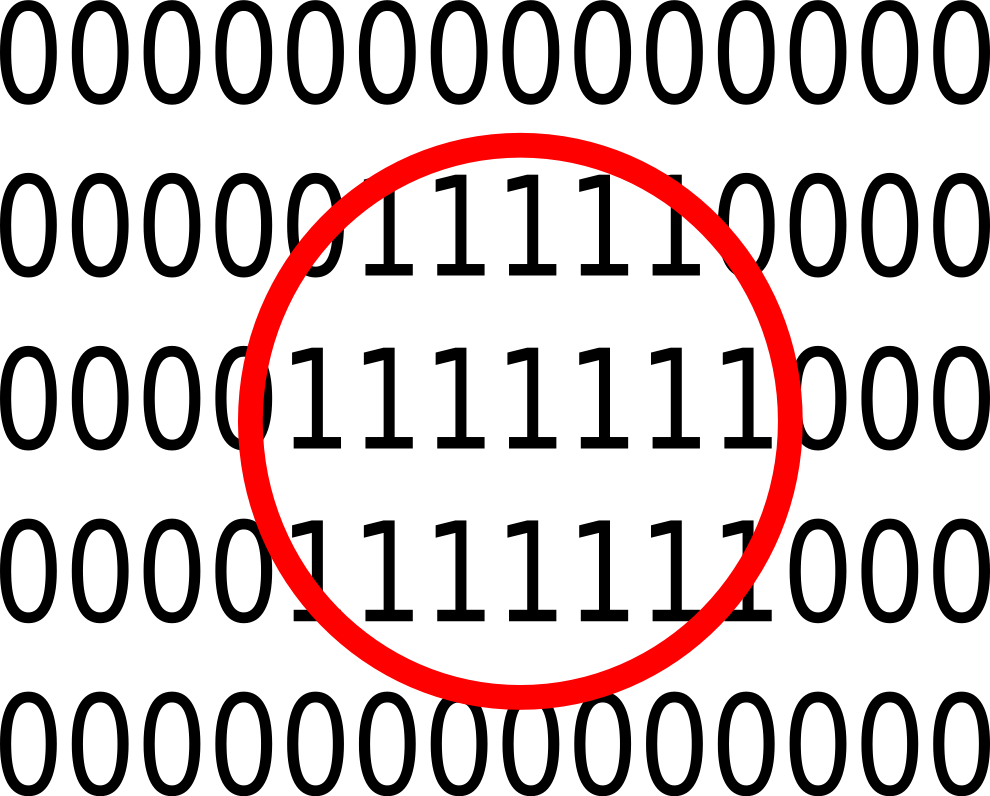
\includegraphics[width=0.45\textwidth]{images/layers2}
	\end{minipage}
	\\\\
	\begin{minipage}[b]{0.48\linewidth}
		\hfill
		\begin{tabular}[b]{|l|l|l|l|}
			\hline
			Layer & Labels \\
			\hline
			\textcolor{red}{red}       & 1 \\
			\hline
		\end{tabular}
	\end{minipage}
	\hspace{0.5cm}
	\begin{minipage}[b]{0.5\linewidth}
		\begin{tabular}[b]{|l|l|l|l|}
			\hline
			Label & Layers \\
			\hline
			1       & \textcolor{red}{red} \\
			\hline
		\end{tabular}
		\hfill
	\end{minipage}
	\caption{One layer\label{fig:layer2}}
\end{figure}



\begin{figure}[ht]
	\begin{minipage}[b]{\linewidth}
		\centering
		\includegraphics[width=0.45\textwidth]{images/layers3}
	\end{minipage}
	\\\\
	\begin{minipage}[b]{0.48\linewidth}
		\hfill
		\begin{tabular}[b]{|l|l|l|l|}
			\hline
			Layer & Labels \\
			\hline
			\textcolor{red}{red}       & 1 \\
			\textcolor{green}{green}       & 2 \\
			\hline
		\end{tabular}
	\end{minipage}
	\hspace{0.5cm}
	\begin{minipage}[b]{0.5\linewidth}
		\begin{tabular}[b]{|l|l|l|l|}
			\hline
			Label & Layers \\
			\hline
			1       & \textcolor{red}{red} \\
			2       & \textcolor{green}{green} \\
			\hline
		\end{tabular}
		\hfill
	\end{minipage}
	\caption{Two non overlapping layers\label{fig:layer3}}
\end{figure}

\begin{figure}[ht]
	\begin{minipage}[b]{\linewidth}
		\centering
		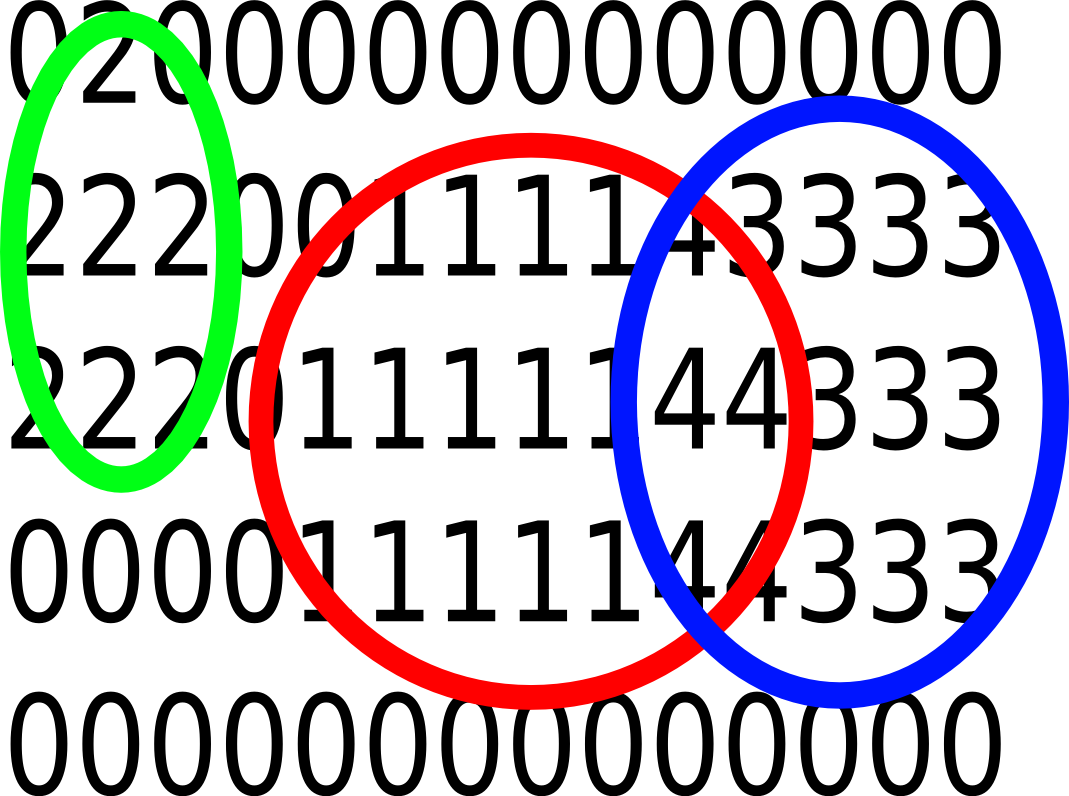
\includegraphics[width=0.45\textwidth]{images/layers4}
	\end{minipage}
	\\\\
	\begin{minipage}[b]{0.46\linewidth}
		\hfill
		\begin{tabular}[b]{|l|l|l|l|}
			\hline
			Layer & Labels \\
			\hline
			\textcolor{red}{red}       & 1, 4 \\
			\textcolor{green}{green}       & 2 \\
			\textcolor{blue}{blue}       & 3, 4 \\
			\hline
		\end{tabular}
	\end{minipage}
	\hspace{0.5cm}
	\begin{minipage}[b]{0.5\linewidth}
		\begin{tabular}[b]{|l|l|l|l|}
			\hline
			Label & Layers \\
			\hline
			1       & \textcolor{red}{red} \\
			2       & \textcolor{green}{green} \\
			3       & \textcolor{blue}{blue} \\
			4       & \textcolor{blue}{blue}, \textcolor{red}{red} \\
			\hline
		\end{tabular}
		\hfill
	\end{minipage}
	\caption{Three layers with one overlap\label{fig:layer4}}
\end{figure}


Our approach has several advantaged over the naive approach. Firstly, creating new layers is memory efficient. Set operations between layers are extremely cheap computationally as only the table that maps labels to layers need to manipulated. Alpha blending overlapping layers during rendering is also extremely efficient and allows for visual comparisons between layers to be performed.

This approach however, can quickly exhaust the available labels should high overlapping between layers occur. The worse scenario is that each newly created layer overlaps with ever other existing label. Should this happen, the number of bits allocated for the label will be the maximum number of layers. For our implementation that is 16 layers. This is however not considered to be a likely scenario. Should no overlapping occur one could have 65536 with 16 bits. The number of layers one an accommodate is equivalent to $2^b/i$ where $b$ is the number of bits used for a label and $i$ i the number of average intersections each layer is expected to have with other layers \todo{Questionable math, needs review}.



\begin{table}[h]
	\begin{center}
	\begin{tabular}{|l|l|l|l|}
	\hline
	Index & X,Y,Z,I (float{[}4{]}) & Label buffer (uint16) & Selection mask (uint8)\\
	\hline
	0     & 0.8, 1.2, 0.2, 0.9 & 0                     & 10000000               \\
	1     & 0.7, 0.5, 0.8, 0.3 & 2                     & 10000000               \\
	2     & 4.3, 0.5, 1.7, 0.9 & 2                     & 10000000               \\
	3     & 0.6, 1.8, 0.1, 0.6 & 1                     & 01000000               \\
	4     & 0.9, 0.5, 0.8, 0.5 & 2                     & 01000000               \\
	5     & 0.1, 0.4, 3.2, 0.9 & 3                     & 01000000               \\
	6     & 2.2, 0.5, 0.3, 0.2 & 5                     & 00000000               \\
	7     & 1.0, 0.9, 0.1, 0.5 & 4                     & 00000000               \\
	\vdots     & \vdots & \vdots  & \vdots             \\
	\hline
	\end{tabular}
	\end{center}
	\caption{GPU point cloud buffer layout}
\end{table}


\begin{table}[h]
	\begin{center}
	\begin{tabular}{|l|l|l|l|}
	\hline
	Layer  name & Color    & Visible & Labels \\
	\hline
	grass       & \#009900 & true & 0, 2, 4      \\
	walls       & \#0000FF & true & 0, 3  \\
	tree        & \#00FF00 & false & 2, 3   \\
	\vdots     & \vdots & \vdots   & \vdots          \\
	\hline
	\end{tabular}
	\end{center}
	\caption{Layer data structure}
\end{table}


\begin{table}[h]
	\begin{center}
	\begin{tabular}{|l|l|l|}
	\hline
	Label & Color  \\
	\hline
	0       & walls.color \\
	1       & grass.color \\
	3       & mix(walls.color, tree.color)	\\
	4       & grass.color	\\
	\vdots     & \vdots      \\
	\hline
	\end{tabular}
	\end{center}
	\caption{GPU label color table}
\end{table}


\section{Undo}
QT based stack
% Technical details of implementation
%!TEX root = thesis.tex
\chapter{Evaluation} \label{ch:eval}

\section{Testing goals}

\begin{itemize}
\item User testing feedback on tools
\item Expert option

\item Correlate feature with segmentation
\item Calculate recall and recognition

\end{itemize}
% Evaluation procedure
% First tried experts in participatory design
% Its bad so we try technology probe (put this in design)
% How participants were recruited
% How bias was avoided

\chapter{Conclusion}


\section{Future work}


\bibliography{thesis}
\bibliographystyle{plainnat}

\end{document}
